\section{Standard Preprocessing} \label{sec:std}

Following the three initial steps presented in \figref{fig:meth:overview} the data needed to undergo multiple preprocessing steps before the images were ready to undergo statistical analysis. There are multiple steps in preprocessing fMRI scans depending on the apparent application and intended outcome. However, there is a standard set of methods that is usually used across all applications. \cite{Moayedi2018} The standard approach to preprocessing of task-related fMRI, which defines a baseline for noise removal, will be described in the following section. The procedures included in the standard preprocessing pipeline can vary depending on the defined study design. In this project the standard preprocessing steps included motion correction, slice timing correction, spatial smoothing and temporal filtering. \Figref{fig:meth:std} provides a chronological overview of the implemented steps in the standard preprocessing pipeline.      

\begin{figure}[H]                 
	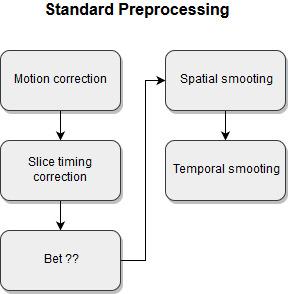
\includegraphics[width=.7\textwidth]{figures/bMethods/Standard_preprocessing} 
	\caption{Flowchart illustrating the chronology of steps in the standard preprocessing pipeline.}
	\label{fig:meth:std} 
\end{figure}

\subsection{Motion correction}

Correcting for motion artifacts when working with fMRI is nearly inevitable, since even the best participants will not be able to hold completely still during acquisition. Even subtle movements such as swallowing will be visible in the acquired image. \cite{Poldrack2011} To correct for these movement induced artifacts, a realignment of all volumes within a scan was carried out using the FSL tool FMRIB's Motion Correction Linear Image Registration Tool (MCFLIRT). \cite{Jenkinson2002}
The tool was used to realign the series of images to a reference image. The volume acquired halfway through the scan was used a reference image. This choice of reference image is often justified by the middle volume being the closest to the average, as well as the scanner at that time would have achieved maximum stability as the magnetization would have reached steady state. \cite{Poldrack2011} The displacement for each voxel in each volume to the voxel in the reference image was calculated and a linear 6 degree of freedom transformation was used to realign the images. The optimal realignment was found by optimizing a the normalized correlation cost function. Due to MCFLIRT only using linear transformation for motion correction only bulk motion was corrected for. \cite{Jenkinson2002}


\subsection{Slice timing correction}

When acquiring fMRI scans the slices in each volume are recorded one by one. This can either be in an ascending, descending or interleaved order. Interleaved order is sequentially skipping every either odd or even slice and then afterwards acquiring the skipped slices. Descending and ascending order are acquired from top to bottom or bottom to top, respectively. Regardless of which order the slices are acquired, a misrepresentation of the hemodynamic response in each slice will be present due to the time difference in which each slice is acquired with. A representation of this effect can be seen in \figref{fig:meth:slice}. The difference in timing for each slice constitutes a problem in the later statistical analyses of the data. The statistical model assumes that all slices are acquired at the same time point. Thereby, the measured signal and the estimated in the statistical model create a mismatch. \cite{Poldrack2011} \\

\begin{figure}[H] 
	{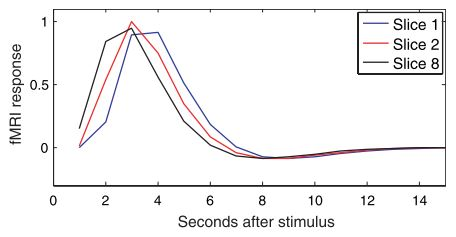
\includegraphics[width=.65\textwidth]{figures/aBackground/response}}  
	\caption{An illustration of the slice-wise acquisition effects of the representation of the hemodynamic response. The response will seem delayed in each slice compared to the previously acquired slice. Illustration taken from \cite{Poldrack2011}.}
	\label{fig:meth:slice}
\end{figure}

As mentioned in \secref{proto} the scan time for one heat run was 386 seconds, and with a TR period of 2 seconds, this resulted in 193 volumes per scan, which needed to undergo slice timing correction. To account for the mismatch in the acquisition time of each slice, slice timing correction was implemented using a FSL tool \cite{FMRIB2018}. This was done by supplying the algorithm with acquisition order and the TR period. As the acquisition order was ascending and the TR-period was two seconds, this was used as input. The slice timing correction worked by shifting the time series for the hemodynamic response curve for each slice in time to fit the middle of the TR period. This was achieved using Hanning windowed sinc interpolation. Choosing the middle slice as the reference introduces the least amount of interpolation, and was therefore seen as the most accurate method. \cite{Poldrack2011} 

%The standard algorithm for slice timing correction uses sinc interpolation between time points, which is accomplished by a Fourier transform of the signal at each voxel. The Fourier transform renders any signal as the sum of some collection of scaled and phase-shifted sine waves; once you have the signal in that form, you can simply shift all the sines on a given slice of the brain forward or backward by the appropriate amount to get the appropriate interpolation. There are a couple pitfalls to this technique, mainly around the beginning and end of your run, highlighted in Calhoun et. al below, but these have largely been accounted for in the currently available modules for slice timing correction in the major programs.
    
%
%\subsection{Brain extraction}
%
%This step is the brain extraction of the brain in the functional scan. The extraction of the functional brain is done in the same way as presented in \secref{BET}. 

\subsection{Spatial smoothing}

Some of the image voxel will likely be contaminated with scattered noise occurring as higher voxel intensities. These can be removed by averaging the misrepresented voxel with its surrounding neighbors. This allows for the possibility of gaining a higher signal-to-noise ratio, however, with the consequence of a decrease in spatial resolution as the image gets more blurred and smaller areas of activation get smeared together. The operation can be justified by the closely neighboring voxel being correlated in effect to the hemodynamic response. Thereby some of the higher-frequency information is removed by spatial smoothing. \cite{Poldrack2011} \\
The implementation of spatial smoothing on the functional image was done using the FSL Smoothing over Univalue Segment Assimilating Nucleus (SUSAN) noise reduction filter. A three dimensional spatial smoothing was carried out on each voxel of the FMRI data set separately. Thereby reducing noise without reducing valid activation, which should be achieved using a default mask size of 5 mm full width half maximum (FWHM) resulted in a trade-off of smoothing both bigger and smaller areas of activation. An advantage of the SUSAN algorithm is its ability to distinguish between tissue types as e.g. grey matter and white matter and thereby only including intensity value from neighboring voxels consisting of the same tissue type as the voxel being smoothened. By applying this technique anatomical structures were preserved and errors in miscalculating the voxel intensity were avoided. \cite{Smith1997}  


\subsection{Temporal filtering}

A common noise component in the fMRI data is the presence of a low-frequency drift. The drift is characterized as a slow increasing trend in the BOLD magnitude, when assessing the signal in the time domain. As mentioned in \secref{ac}, the frequency of noise was 0 Hz to 0.015 Hz and the frequency band of activation was approximately 0.025 Hz. To dampen some of the low-frequency artifactual content a high-pass filter with a cutoff frequency of 0.01 Hz was implemented. \cite{FMRIB2018} \\


 
 % The reason for this type of noise contamination has been heavily investigated, and conclusions state that the noise originates from MRI scanner instability. As this low-frequency drift will always be present, it is very crucial to consider the interval of which tasks or stimuli are performed to avoid the output being present in the noise range of $0$ to $0.015$ Hz. Therefore stimuli or tasks should be performed within intervals of $70$ s or less. \cite{Poldrack2011} \\ 
 
 
 
 
